\documentclass[a4paper,
    11pt,
    headings=small,
    ngerman,
    listof=totoc,
    index=totoc,
    numbers=noenddot]{scrreprt}[2021/11/13]
\usepackage{ifxetex,ifluatex}
\ifcase \ifxetex 1\else\ifluatex 1\else 0\fi\fi\usepackage[utf8]{inputenc}\fi
\usepackage[T1]{fontenc}
\usepackage[ngerman]{babel}
\usepackage[utf8]{inputenc}
\usepackage{setspace}
\onehalfspacing
\usepackage{lmodern}
\usepackage{csquotes}

%%% Kopfzeile %%%
% \clearmainofpairofpagestyles
% \pagestyle{scrheadings}
% \renewcommand*{\chapterpagestyle}{scrheadings}
% \automark[chapter]{chapter}
% \renewcommand*{\headfont}{\normalfont}
% \setkomafont{pageheadfoot}{}
% \renewcommand*{\sectionmarkformat}{} 

\usepackage[automark,headsepline=.4pt]{scrlayer-scrpage}
\clearmainofpairofpagestyles
\pagestyle{scrheadings}
\renewcommand*{\chaptermarkformat}{%
	\chaptername~\thechapter\autodot\enskip}
% \ohead*{\pagemark}
\ihead{\headmark}
% \setkomafont{pageheadfoot}{\normalfont}
\setkomafont{pageheadfoot}{}
\renewcommand*{\sectionmarkformat}{}
\cfoot{\pagemark}
\footskip1cm

\usepackage[left=2.5cm,right=2.5cm,top=3cm,bottom=2.5cm]{geometry}
 
\usepackage{makeidx}\makeindex% Nur als Beispiel

\usepackage{xcolor, soul}
\definecolor{codebackground}{rgb}{0.95, 0.95, 0.92}
\definecolor{Black}{rgb}{0, 0, 0}

%%% Für Abkürzungen und Abkürzungsverzeichnis %%%
\usepackage[printonlyused,withpage]{acronym}

%%% Für Quotes %%%
\usepackage{url}
\usepackage[ngerman]{varioref}
\usepackage{mwe}
\usepackage{hyperref}% Weil es so in der Frage enthalten war.
 \hypersetup{%draft, 								% no hyperlinking at all (useful in b/w printouts)
    colorlinks=true, breaklinks=true,
    urlcolor=Black, linkcolor=Black, citecolor=Black,
    linktoc=page, %
    bookmarksnumbered, bookmarksopenlevel=1, bookmarksdepth = section,%
    pdfstartview=FitV,
    }
\setlength{\parindent}{0em}
\usepackage{bookmark}% Weil das hyperref deutlich verbesser.
\usepackage{cleveref}
\crefname{paragraph}{Abschnitt}{Abschnitt}

%%% Für Textübergreifende Numerierung %%%
\usepackage{enumitem}
\renewcommand{\labelenumi}{\alph{enumi})}

%%% Um PDFs einzubinden %%%
\usepackage{pdfpages}

%%% Um Zahlen mit Einheiten korrekt darstellen %%%
\usepackage{siunitx}
\sisetup{
  locale = DE ,
  detect-all,
  binary-units = true
}

%%% Code schoen darstellen %%%
\usepackage{listings}
\lstdefinestyle{MyPythonStyle}{
  frame=tb, % hrule above and below
  keepspaces=true,
  breaklines=true,
  columns=flexible,
  basicstyle=\texttt\scriptsize,
  escapeinside={(*@}{@*)}, % for escaping
  backgroundcolor=\color{codebackground},
  showstringspaces=false,
  language=Python,
  keywordstyle=\color{blue},
  stringstyle=\color{red},
  commentstyle=\color{teal},
  numbers=left, % {none, left, right}
  firstnumber=1,
  numberstyle=\scriptsize\color{black},
  numbersep=5pt,
  xleftmargin=5.0ex,
  gobble=-4
}

%%% Korrekte darstellung fuer Sonderzeichen im Code
\lstset{literate=%
    {Ö}{{\"O}}1
    {Ä}{{\"A}}1
    {Ü}{{\"U}}1
    {ß}{{\ss}}1
    {ü}{{\"u}}1
    {ä}{{\"a}}1
    {ö}{{\"o}}1
    {~}{{\textasciitilde}}1
}


%%% Verzeichnisse im Anhang %%%
\DeclareNewTOC[%
  owner=\jobname,
  listname={Inhalt des Anhangs},% Titel des Verzeichnisses
]{atoc}% Dateierweiterung (a=appendix, toc=table of contents)
\DeclareNewTOC[%
  listname={Abbildungen im Anhang},% Titel des Verzeichnisses
]{alof}% Dateierweiterung (a=appendix, lof=list of figures)
\DeclareNewTOC[%
  listname={Tabellen im Anhang},% Titel des Verzeichnisses
]{alot}% Dateierweiterung (a=appendix, lot=list of tables)
 
\makeatletter
\newcommand*{\useappendixtocs}{%
  \renewcommand*{\ext@toc}{atoc}%
  \scr@ifundefinedorrelax{hypersetup}{}{% damit es auch ohne hyperref funktioniert
    \hypersetup{bookmarkstype=atoc}%
  }%
  \renewcommand*{\ext@figure}{alof}%
  \renewcommand*{\ext@table}{alot}%
}
\newcommand*{\usestandardtocs}{%
  \renewcommand*{\ext@toc}{toc}%
  \scr@ifundefinedorrelax{hypersetup}{}{% damit es auch ohne hyperref funktioniert
    \hypersetup{bookmarkstype=toc}%
  }%
  \renewcommand*{\ext@figure}{lof}%
  \renewcommand*{\ext@table}{lot}%
}
\scr@ifundefinedorrelax{ext@toc}{%
  \newcommand*{\ext@toc}{toc}
  \renewcommand{\addtocentrydefault}[3]{%
    \expandafter\tocbasic@addxcontentsline\expandafter{\ext@toc}{#1}{#2}{#3}%
  }
}{}
\makeatother
 
\usepackage{xpatch}
\xapptocmd\appendix{%
  \addpart{\appendixname}
  \useappendixtocs
}{}{}

%%% Alles bzgl. des Literaturverzeichnisses
\usepackage[bibencoding=utf8,
			sortlocale=de,
			style=numeric,
			pagetracker=true,
			autocite=inline,
			backrefstyle=three+,
			date=short,
			sorting=nty,
			backend=biber]{biblatex}
\bibliography{Literaturverzeichnis}

%%% urldate in eckigen Klammern %%%
\DeclareFieldFormat{urldate}{\mkbibbrackets{#1}}
%%% URL: = Verfügbar unter: %%%
\DeclareFieldFormat{url}{{Verfügbar unter:}\space\url{#1}}
%%% Abstand zwischen den Literaturangaben %%%
\setlength{\bibitemsep}{1.3em}
%%% statt und ein & %%%
\renewcommand*{\finalnamedelim}{\space\&\space}
%%% Nachname, Vorname, immer %%%
\DeclareNameAlias{sortname}{last-first}
 
 
\begin{document}

%%% Titelblatt %%% 
\pagenumbering{gobble}
\pagestyle{empty}


\begin{center}
  \Large{Berufliches Schulzentrum für Elektrotechnik Dresden}\\
\end{center}

\begin{center}
  \Large{Fachbereich Informationstechnik}
\end{center}
\begin{verbatim}

\end{verbatim}
\begin{center}
  \textbf{\LARGE{Vorlage Abschlussarbeit}}
\end{center}

\begin{center}
  \Large{Kleine, nicht perfekte Vorlage fuer die IHK Abschlussarbeit}
\end{center}

\vspace{\fill}
\begin{flushleft}
  \begin{tabular}{lll}
    \textbf{erstellt von:} & Johannes Leyrer \flq{}i20leyrerjo@bszetdd.lernsax.de\frq{}   \\
                           &                                                            & \\
    \textbf{erstellt im:}  & Lehrjahr 2, 2021/2022                                        \\
                           &                                                            & \\
    \textbf{betreut von: } & Mama Musterfrau                                              \\
                           &                                                            & \\
                           &                                                            & \\
  \end{tabular}
\end{flushleft}

\begin{description}
  \item[Disclaimer:] Diese Vorlage ist nicht offiziell. Insbesondere erhebe ich keinen Anspruch auf Vollständigkeit oder Korrektheit. Ich bin jederzeit froh um Hinweise zu Fehlern oder Unklarheiten.
\end{description}

\newpage


\includepdf[pages={1}]{PDFs/Projektantrag.pdf}

\newpage

%%% Inhaltsverzeichnis %%%
\tableofcontents
\cleardoublepage

\newpage
%%% Kopfzeile
\pagestyle{scrheadings}
\pagenumbering{arabic}

\chapter{Ueberschrift auf Ebene 0}

\section{Beispielstext}\label{sec:bsp}

Hier ist ein Beispiel für ein Zitat: \glqq Zitat\grqq{} \cite{Bernhardi.1883}.

Hier ist ein Verweis auf einen \cref{sec:bsp}.

Hier ist die Verwendung von Abkürzungen: Das Backend wird von einem \ac{API} betrieben. Diese acp{API} sind ein grosser Teil der Systemlandschaft. \acp{API} sind in der Informatik nicht wegzudenken. Ein \ac{API} ist ein wichtiges Werkzeug. Anders als das Backend ist das Frontend meist mittels \ac{HTML} und \ac{CSS} aufgebaut. \ac{HTML} ist inzwischen mit der Versionsnummer 5 vertreten.

\subsection[Kurzbeschreibung]{Beispiel für ein Unterkapitel}

\newpage

\subsection{Hier ist ein Bild}

%%% [here, top, bottom, (new) page]
%%% width= prozentual der Textbreite
\begin{figure}[htbp]
  \centering
  
\includegraphics[width=0.7\textwidth]{pics/bszet.png}
  \caption{Logo BSZ ET Dresden}
  \label{fig:logobszetdd}
\end{figure}


\subsection{Hier ist eine Tabelle}

\begin{table}[h]
  \centering
  \renewcommand{\arraystretch}{1.25}
  \caption{Test Tabelle}
  \begin{tabular}{lcr|p{5cm}}
    links & mitte & rechts & bestimmter Abstand erzwungen \\
    \hline
    1     & 2     & 3      & 4                            \\
  \end{tabular}
  \label{tab:testtabelle}
\end{table}


\subsection{Hier ist ein bisschen Code}

\begin{lstlisting}[caption={Spalten in numpy}, style=MyPythonStyle]
  import numpy as np

  vals = np.random.rand(4, 4)
  # Getting the first and the third row of the matrix
  vals[::2]
\end{lstlisting}


\newpage
\printbibliography[keyword=Quelle,title={Quellenangabe},heading=bibintoc]

\newpage
%%% Abkürzungsverzeichnis %%%
\chapter*{Abkürzungsverzeichnis}
\addcontentsline{toc}{chapter}{Abkürzungsverzeichnis}
%%% in [] sollte die längste Abkürzung stehen, damit die Ausrichtung ordentlich ist
\begin{acronym}[HTML]
  \acro{API}{Application Programming Interface}
  \acroplural{API}[APIs]{Application Programming Interfaces}
  \acro{CSS}{ Cascading Style Sheets}
  \acro{HTML}{Hypertext Markup Language}
  \acro{SQL}{Structured Query Language}
\end{acronym}

%%% Abbildungsverzeichnis
\listoffigures
%%% Tabellenverzeichnis
\listoftables
%%% Codeverzeichnis
\lstlistoflistings


\newpage
\pagestyle{scrheadings}
\appendix
\listofatocs
\newpage

\begin{figure}[htbp]
  \centering
  
\includegraphics[width=0.5\textwidth]{pics/bszet.png}
  \caption{Logo BSZ ET Dresden}
  \label{fig:logobszetddappendix}
\end{figure}

\begin{table}[h]
  \caption{test-tab-appendix}
  \noindent
  \centering
  \begin{tabular}{|c|c|}
    \hline
    a & b\tabularnewline
    \hline\hline
    1 & 2\tabularnewline
    \hline
  \end{tabular}
\end{table}

\newpage
%%% Abbildungsverzeichnis im Anhang
\listofalofs

\newpage

%% Tabellenverzeichnis im Anhang
\listofalots

\newpage

\addcontentsline{toc}{chapter}{Kundendokumentation}
%%% Kundendokumentation aus extra Datei %%%
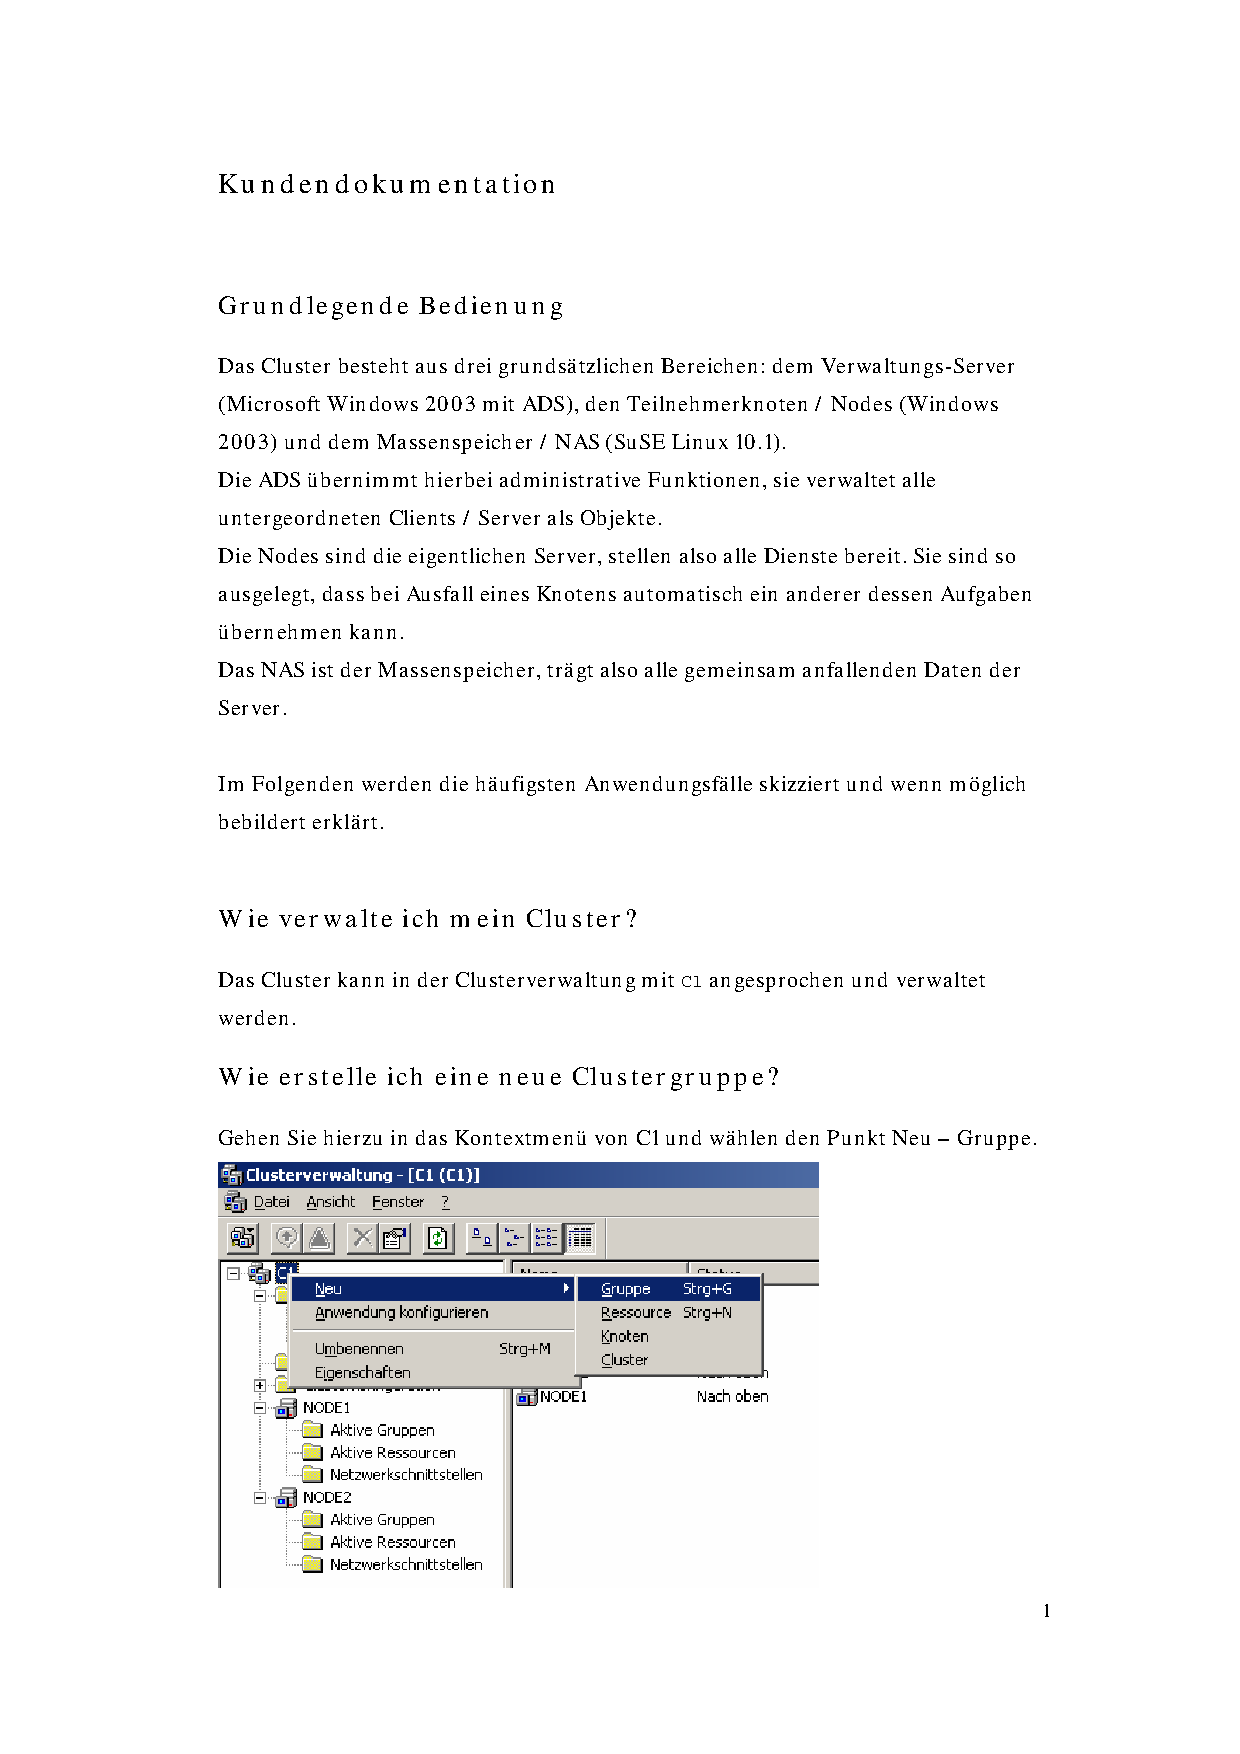
\includepdf[pages=-]{PDFs/Kundendokumentation.pdf}

\end{document}

